\documentclass[a4paper,12pt]{book}
\usepackage{amsmath}
\usepackage{amssymb}
\usepackage[utf8]{inputenc}
\usepackage[T1]{fontenc}
\usepackage[francais]{babel}
\usepackage{graphicx}
\usepackage[colorlinks]{hyperref}
\usepackage{imakeidx}
\usepackage{lipsum} 
\usepackage{a4wide}
\usepackage{svg}

\makeatletter
\providecommand*{\input@path}{}
\edef\input@path{{chapitres/}\input@path}% prepend
\makeatother



\title{Les notes de Rancune: \\Electronique Analogique}
\author{Rancune}
\date{\today}

\makeindex

\begin{document}

\maketitle

\frontmatter

\tableofcontents    

%\chapter*{Introduction}
\addcontentsline{toc}{part}{Introduction}


\mainmatter

\part{ Les lois de base }

\chapter{Les grandeurs électriques}

\section{La charge électrique}

\begin{tabular}{ll}
\textbf{Notation usuelle~:} & $Q$, $q$ \\
\textbf{Unité~:} & Coulomb (C) \\
\textbf{Unité SI~:} & $A \cdot s $ \\
\textbf{Nature~:} & Grandeur scalaire \\
\end{tabular} 

\subsection*{Définition}

\index{charge!charge electrique@charge électrique}

Tout comme la masse pour les interactions gravitationnelles, la \textbf{charge électrique} est une propriété fondamentale de la matière qui lui permet d'intéragir par le biais de champs électromagnétiques. \\ 

Il existe deux types de charges électriques : les charges positives ($+$) et les charges négatives ($-$). Deux charges de même signe se repoussent, deux charges de signes différents s'attirent.\\

On appelle \textbf{porteur de charge} une particule ou un corps portant une charge non nulle. Bien qu'on pense en général aux électrons lorsqu'on parle de courant électrique, ceux-ci ne sont pas les seuls porteurs de charges. Les protons et les ions (anions et cations), par exemple, en sont également. 

\index{charge!porteur de charge}

\subsection*{ Quantification de la charge~: }

\textbf{La charge électrique est quantifiée} : elle est un multiple entier de la \textbf{charge élémentaire} $e$, qui correspond à la charge d'un électron.
\index{electron@électron}
\index{charge!charge elementaire@charge élémentaire}
\index{charge!quantification de la charge}

\begin{equation}
	e \approx 1,602.10^{-19} C
\end{equation}

Néanmoins, on la considère en général en électronique comme une grandeur continue. Ceci a pour conséquence d'introduire dans les calculs un bruit particulier, appelé "bruit de grenaille".
\index{bruit!bruit de grenaille}
\index{grenaille!bruit de grenaille}

\subsection*{ Conservation de la charge~: }

\textbf{La charge électrique est une grandeur conservative}~: la charge d'un système isolé est invariante. La charge electrique ne peut donc être qu'échangée avec un autre système, mais ni créée, ni annihilée.
\index{charge!conservation de la charge}

\section{Le potentiel}

\begin{tabular}{ll}
\textbf{Notation usuelle~:} & V \\
\textbf{Unité~:} & Volt (V)\\
\textbf{Unité SI~:} & ${kg} \cdot m^2 \cdot {s}^{-3} \cdot A^{-1}$ \\
\textbf{Nature~:} & Grandeur scalaire \\ 
\end{tabular}

\subsection*{Définition}

En tout point de l'espace est défini un \keyword{potentiel}. Cette valeur scalaire correspond à l'énergie potentielle électrostatique que posséderait une charge électrique unitaire située en ce point. \\ 

Les points possédant une même valeur de potentiel sont désignés sous le nom d'\textbf{équipotentielle}.\index{equipotentielle@équipotentielle}

\subsection*{La terre}

Le \textbf{potentiel zéro} est par convention le potentiel de la \textbf{terre}, obtenu en plantant un piquet conducteur en terre. On le suppose en général égal en tout lieu mais c'est une approximation. \\

Cet équipotentiel zéro est noté avec le terme anglais "Ground" (ou GND en abbrégé) dans les circuits. On le représente avec le symbole suivant~:

\begin{figure}[!h]
\centering
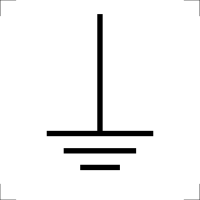
\includegraphics{part01/chap01/ground.png}
	\caption{Symbole représentant la terre \\ norme IEC 60417 }
\end{figure}

\index{terre}
\index{ground}

\section{La tension}

\begin{tabular}{ll}
\textbf{Notation usuelle~:} & $U$, $u$, $U_{AB}$ \\
\textbf{Unité~:} & Volt (V) \\
\textbf{Unité SI~:} & ${kg} \cdot m^2 \cdot {s}^{-3} \cdot A^{-1}$ \\
\textbf{Nature~:} & Grandeur scalaire \\
\end{tabular} 

\subsection*{Définition}

Une \keyword{tension} $U_{AB}$ est la circulation du champs électrique le long d'un circuit $\mathscr{C}$ entre les points $A$ et $B$~:

\begin{equation}
	U_{AB} = \int_{\mathscr{C}_{A}}^{\mathscr{C}_B}\vec{E}\,dl
\end{equation}

Cependant, cette définition est trop détaillée pour l'électronique. En effet, si l'on suppose que le temps de propagation des ondes électromagétiques est négligeable (hypothèse du régime stationnaire), la tension est alors égale à la "\textbf{différence de potentiel}" entre les deux extrémités du circuit.

\begin{equation}
	U_{AB} = V_A - V_B
\end{equation}

\index{potentiel!difference de potentiel@différence de potentiel}

\subsection*{Représentation graphique: }

\begin{minipage}{7cm}
\begin{center}
\includesvg{part01/chap01/tension}
\end{center}
\end{minipage}
\hspace{1cm}
\begin{minipage}{7cm}
Une tension est représentée par une flêche. Son sens est important car une tension est une \underline{grandeur signée}. 
\end{minipage}\\

\subsection*{Mesure d'une tension}

En électronique, une tension se mesure toujours \emph{entre deux points}, à l'aide d'un voltmètre (ou d'un oscilloscope si on veut en voir les variations temporelles). \\


\begin{minipage}{7cm}
\begin{center}
\includesvg{part01/chap01/mesure_tension}
\end{center}
\end{minipage}
\hspace{1cm}
\begin{minipage}{7cm} 
	Le voltmètre se connecte en parallèle de la tension à mesurer. 
\end{minipage}\\

\section{Le courant}

\begin{tabular}{ll}
\textbf{Notation usuelle~:} & $I$, $i$ \\
\textbf{Unité~:} & Ampère (A) \\
\textbf{Unité SI~:} & $A$ \\
\textbf{Nature~:} & Grandeur scalaire \\
\end{tabular} 

\subsection*{Définition}

Un \textbf{courant} est un mouvement d'ensemble de porteurs de charges électriques au sein d'un matériau conducteur. Ces porteurs de charge sont dans le cas le plus courant des électrons, mais cela peut également être des ions positifs ou négatifs (Par exemple dans le cas des electrolytes) ou encore n'importe quel corps portant une charge non nulle. 

\index{courant!courant électrique}

\subsection*{ Représentation graphique: }

\begin{minipage}{7cm}
	\includesvg{part01/chap01/courant} 
\end{minipage}
\hspace{1cm}
\begin{minipage}{7cm}
	Le courant électrique est généralement représenté par une flêche située sur le circuit. Son sens est important car un courant est une \underline{grandeur signée}. 
\end{minipage}\\

\subsection*{Mesure d'un courant électrique }

En pratique, un courant se mesure généralement à l'aide d'un ampèremètre. \\ 

\begin{minipage}{7cm}
\begin{center}
\includesvg{part01/chap01/mesure_courant}
\end{center}
\end{minipage}
\hspace{1cm}
\begin{minipage}{7cm} 
	L'ampèremètre se connecte en série sur le circuit dans lequel on veut mesurer un courant. 
\end{minipage}\\

\index{courant!mesure du courant}
\index{amperemetre@ampèremètre}

\subsection*{ Sens conventionnel du courant: }

Par convention, le courant sort du générateur électrique par la borne positive et y revient par la borne négative. C'est ce que l'on appelle le \textbf{sens conventionnel du courant}. \\
\index{courant!sens conventionnel du courant}
\index{conventionnel!sens conventionnel du courant}

On ne raisonne jamais en électronique en utilisant le sens réel des porteurs de charges, car celui-ci sera différent s'il s'agit d'électrons (qui circulent du pôle négatif vers le pôle positif du générateur) ou de cations (qui circulent en sens inverse). Cela n'a aucune importance et ne ferait que complexifier inutilement les raisonnements. Dans la suite de ce document, et plus largement dans l'intégralité des ouvrages lus par votre serviteur, c'est toujours le sens conventionnel qui est utilisé.

\subsection*{Intensité du courant}

L'\keyword{intensité} du courant électrique (parfois appelée "\keyword*{ampérage}" ou "\keyword*{courant}") correspond au débit de charges électriques à travers une surface donnée (le plus souvent la section d'un fil électrique)~: 

\begin{equation}
	i(t) = \dfrac{dq}{dt} 
\end{equation}

avec~: \\
\begin{itemize}
	\item[$\bullet$] $i$ : l'intensité du courant
	\item[$\bullet$] $q$ : la charge électrique
	\item[$\bullet$] $t$ : le temps.
\end{itemize}

\section{L'énergie électrique}

\begin{tabular}{ll}
\textbf{Notation usuelle~:} & $E$ \\
\textbf{Unité~:} & Joule (J) \\
	\textbf{Unité SI~:} & $kg \cdot m^2 \cdot s^{-2}$ \\
\textbf{Nature~:} & Grandeur scalaire \\
\end{tabular} 

\subsection*{Définition}

\textbf{Parler d'énergie électrique est au sens strict un abus de langage}. Ce n'est pas une véritable forme d'énergie comme peuvent l'être l'énergie cinétique ou l'énergie potentielle. Il s'agit plutôt d'un vecteur énergétique, c'est à dire un moyen de transférer de l'énergie entre deux systèmes : l'électricité requiert et transporte de l'énergie.\\
\index{energie@énergie}

L'énergie électrique est définie de la façon suivante~:

\begin{equation}
	E = q \cdot U
\end{equation}

avec~:\\
\begin{itemize}
	\item[$\bullet$] $E$ la quantité d'énergie en joules
	\item[$\bullet$] $q$ la charge électrique en coulombs
	\item[$\bullet$] $U$ la tension électrique en volts
\end{itemize}

\subsection*{Autre unité de mesure}

Le joule étant une unité de mesure assez petite pour les besoins des électriciens, une autre unité est souvent utilisée~: le kiloWattheure (kWh). 
\index{kiloWattheure}

$$ 1\:kWh = 10^3 \cdot 3600\:J = 3.6\:MJ $$


\subsection*{Lien avec la puissance}

si $I$ est le courant, la quantité de charges qui circulent pendant un temps $\Delta t$ est~: 

$$q = I \cdot \Delta t$$

(On suppose le courant constant pendant l'intervalle de temps).\\

La quantitée d'énergie échangée $E$ pendant $\Delta t$ est donc~:

$$ E = q \cdot U = I \cdot \Delta t \cdot U = U \cdot I \cdot \Delta t $$

Ce qui amène à~: \\
\begin{equation}
E = P \cdot \Delta t 
\end{equation}

avec $P$ la puissance électrique.

\section{La puissance électrique}

\begin{tabular}{ll}
\textbf{Notation usuelle~:} & $P$ \\
\textbf{Unité~:} & Watt (W) \\
	\textbf{Unité SI~:} & $kg \cdot m^2 \cdot s^{-3}$ \\
\textbf{Nature~:} & Grandeur scalaire \\
\end{tabular} 

\subsection*{Définition}

\textbf{La puissance électrique}\index{puissance!puissance electrique@puissance électrique} est un taux d'énergie transférée par un circuit électrique par unité de temps. La puissance est donc reliée à l'énergie échangée par la relation~:

\begin{equation}
	P = \dfrac{E}{\Delta t}
\end{equation}

Ce qui nous permet également de l'exprimer en fonction de la tension et du courant :

\begin{equation}
	P = U \cdot I
\end{equation}

Pour un générateur, cette quantité est négative (le générateur fournit de l'énergie). Pour une charge, cette quantité est positive.


%\input{ lois_électriques.tex }
%\input{ résistance.tex }
%\input{ capacité.tex }
%\input{ inductance.tex }

%\part{ Les composants passifs }

%\input{ resistor.tex }
%\input{ condensateur.tex }
%\input{ bobine.tex}

%\part{ Les semi-conducteurs }

%\input{ diode.tex }
%\input{ bjt.tex }
%\input{ fet.tex }

%\part{ Analyse harmonique }

% Les annexes

%\appendix

%\backmatter

\printindex

% Fin du document
\end{document}

